\documentclass[article,a4paper,12pt,brazil,sumario=tradicional]{abntex2}
\usepackage{titlesec}

\setcounter{secnumdepth}{4}

\titleformat{\paragraph}
{\normalfont\normalsize}{\theparagraph}{1em}{}

\usepackage{array}
\usepackage{subfig}
\usepackage[utf8]{inputenc}
\usepackage{indentfirst}
\usepackage{hyperref}
\usepackage[hyphenbreaks]{breakurl}
\usepackage[alf,abnt-etal-text=it]{abntex2cite}
\usepackage[brazil]{babel}
\usepackage[space]{grffile}
\graphicspath{ {./images/} }
\setlength{\parindent}{3em}

\newcolumntype{C}[1]{>{\centering\arraybackslash\hspace{0pt}}p{#1}}

\setlrmarginsandblock{3cm}{3cm}{*}
\setulmarginsandblock{3cm}{2cm}{*}
\checkandfixthelayout

\titleformat{\section}{\normalfont\normalsize\bfseries}{\thesection.}{1em}{\MakeUppercase}
\titleformat{\subsection}{\normalfont\normalsize}{\thesubsection.}{1em}{\MakeUppercase}
\titleformat{\subsubsection}{\normalfont\normalsize\bfseries}{\thesubsubsection.}{1em}{}

\renewenvironment{quotation}
  {\small\list{}{\rightmargin=0cm \leftmargin=2cm}%
   \item\relax}
  {\endlist}
  
\hypersetup{%
    pdfborder = {0 0 0}
}

\title{ {\Large Revalidação de análise de performance (Mbips e iops) entre lustre e sistemas de armazenamento compatíveis com s3\footnote{Trabalho de conclusão de curso apresentado ao curso de Bacharelado em Ciência da Computação da Universidade Federal Fluminense como requisito parcial para conclusão do curso.}\\\\
\vspace{.2} 
\textit{Revalidation of performance analysis (Mbips and Iops) between Lustre and S3-compatible storage systems}\\}}

\date{ }

\begin{document}

\textual

\begin{center}
{\Large Revalidação de análise de performance (Mbips e iops) entre lustre e sistemas de armazenamento compatíveis com s3\footnote{Trabalho de conclusão de curso apresentado ao curso de Bacharelado em Ciência da Computação da Universidade Federal Fluminense como requisito parcial para conclusão do curso.}

\textit{Revalidation of performance analysis (Mbips and Iops) between Lustre and S3-compatible storage systems}\\}
\end{center}
\vspace{.2cm} 

\begin{flushright}
João Pedro Abreu de Souza\footnote{Graduando do Curso de Ciência da Computação - UFF, jp\_abreu@id.uff.br}

Lúcia Maria de Assumpção Drummond\footnote{Orientador - Instituto de Computação - UFF, lucia@ic.uff.br} 
\end{flushright}

\vspace{\onelineskip}

\begin{center}
    \textbf{Resumo}
\end{center}

\vspace{-.3cm}

\noindent Utilizando dois benchmarks padrão(io-500 e md-workbench) para analisar a evolução da performance relativa entre
sistemas de armazenamento típicos de hpc (lustre, um sistema de arquivos paralelo) e sistemas de armazenamento baseados
nas APIs rest do s3 e na API da libs3, busquei verificar se houve melhora desde 2021, ano que foi publicado um artigo realizando
uma comparação entre ambos os sistemas de armazenamento. A reavaliação se sustenta no fato do artigo ter 2 anos, e nesse
tempo o s3 recebeu várias mudanças e manteve a mesma API, logo sendo possível avaliar se a distância entre ele e o lustre
permanece a mesma. O lustre utilizado foi o provisionado pelo serviço fsx da aws e o s3 sendo o serviço da própria aws. O resultado foi ...

\vspace{.4cm}
 
\noindent
\textbf{Palavras-chaves}: HPC; Lustre; S3; AWS.
 
\vspace{\onelineskip}

\begin{center}
    \textbf{Abstract}
\end{center}

\vspace{-.3cm}
\begin{hyphenrules}{english}
\noindent Using two standard benchmarks(io-500 and md-workbench) to analyze the evolution of relative performance between
typical hpc storage systems (lustre, a parallel file system) and storage systems based
in the rest APIs of s3 and the libs3 API, I sought to check whether there was an improvement since 2021, the year in which an article was published
a comparison between both storage systems. The reevaluation is based on the fact that the article is 2 years old, and in this
Over time, s3 received several changes and maintained the same API, making it possible to assess whether the distance between it and the chandelier
remains the same. The lustre used was the one provisioned by the aws fsx service and the s3 being the aws service itself. The result was ...
\end{hyphenrules}
\vspace{.4cm}
 
\noindent \textbf{Keywords}: HPC; Lustre; S3; AWS.

\vspace{.4cm}

\noindent \textbf{Aprovado em:} dd/mm/aaaa.~~~\textbf{Versão Final em:} dd/mm/aaaaComo visto na figura~\ref{fig:lustre}., 

\begin{figure}[!ht]
	\centering
	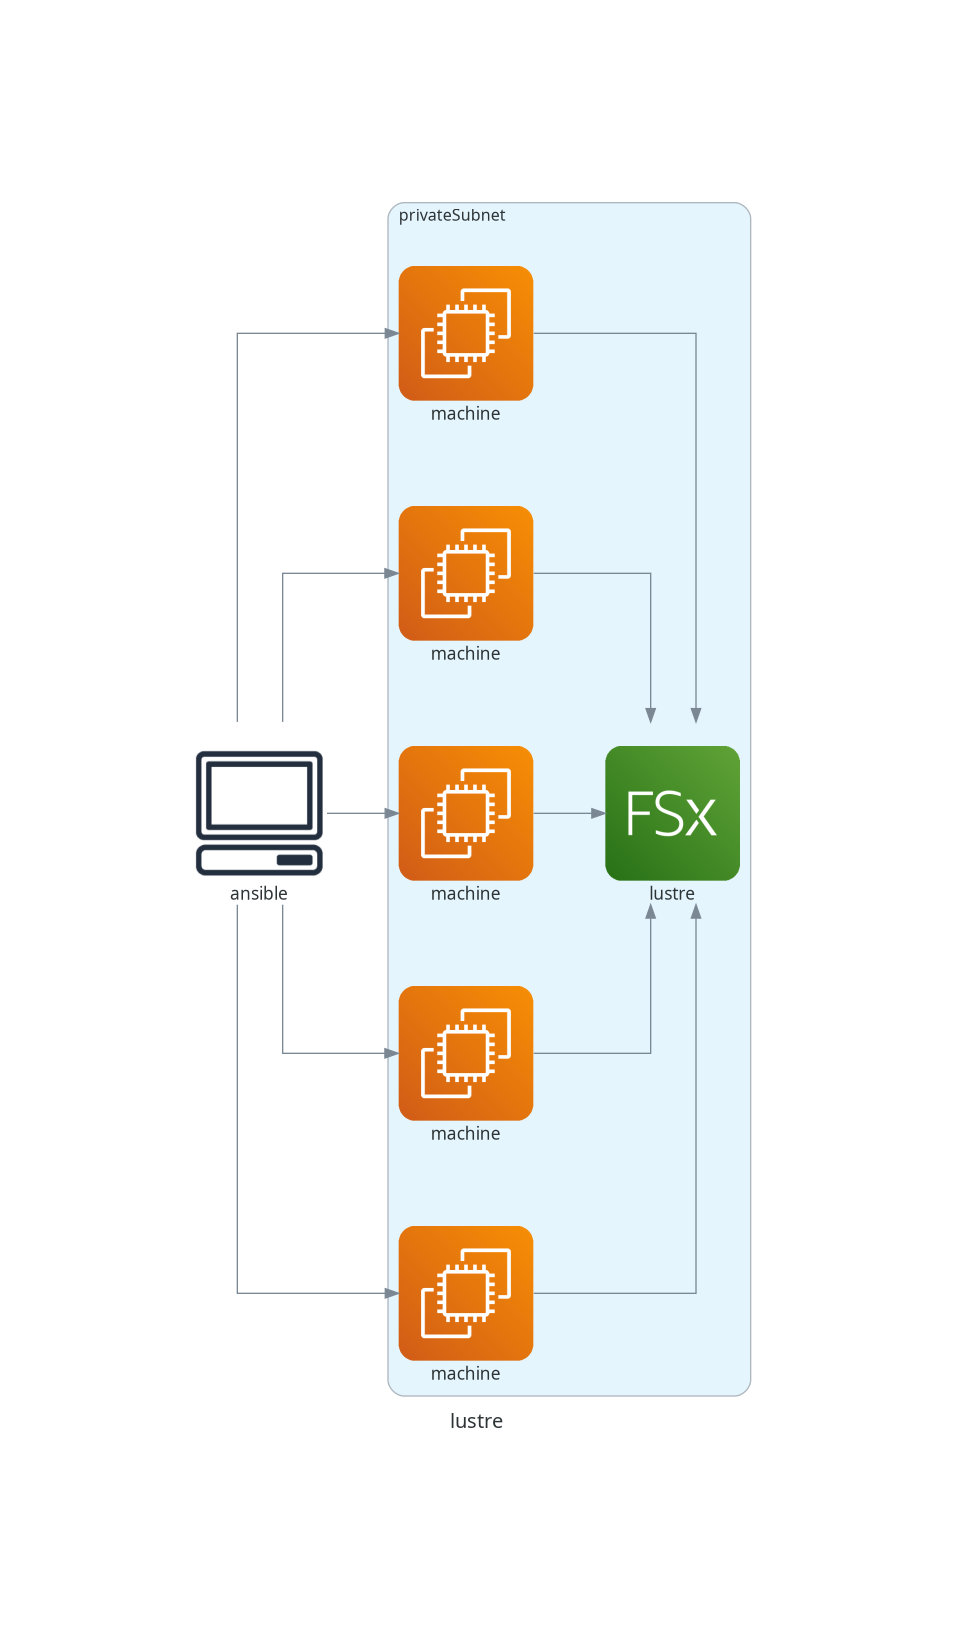
\includegraphics[width=1\textwidth]{lustre.png}
	\caption{Arquitetura do cluster usando lustre Fonte: fornecido pelo autor.}
	\label{fig:lustre}
\end{figure}

\section{Introdução}

HPC é utilizado para computar uma grande gama de problemas, que mesmo uma única maquina poderosa não seria capaz em tempo hábil (i.e. Resolução de sistemas de equações parciais em uma grande malha para simulação). Normalmente as aplicações HPC são escritas em C ou Fortran, e rodam em super-computadores dedicados a essa função, como o mistral, super-computador alemão.

Desde a criação da AWS, em 2006, as plataformas de computação com modelo elastico, pagando pelo uso, vulgo nuvem, se tornaram a norma no desenvolvimento de aplicações, chegando até mesmo a areas altamente reguladas como o setor de pagamentos. Por conta disso, pesquisadores buscavam verificar se a nuvem poderia suportar os workflows de aplicações HPC. Nesse contexto, o artigo de 2021, "analyzing the performance of the S3 Object Storage API for HPC Workloads", foi tomado como base para realização desse trabalho, buscando avaliar as mudanças nos resultados que possam ter advindo nesses dois anos. Para isso, utilizei o io500, benchmark ior e mdtest, dado que o find, outro benchmark fornecido pelo io500, não é suportado para uso com o s3.

\section{Desenvolvimento}

\subsection{Lustre - baseline}
Como visto na figura~\ref{fig:lustre}., a arquitetura utilizada contém 2 sub-redes, uma privada e uma pública, com as maquinas da subnet privada acessando o lustre provisionado via o serviço fsx da propria AWS. Isso garante que o teste não será influenciado por falhas no provisionamento do cluster. Essa arquitetura foi pensada pois a conexão direta entre as maquinas e o lustre, que exige uma interface de rede, não é possivel enquanto se mantém um ip publico. O teste foi executado com script runTcc.sh, com seu código em anexo. Os resultados foram

\begin{table}[htb]
	\begin{tabular}{|l|l|l|}
		\hline
		& mdtest & ior \\ \hline
		ior-easy-write    &        &     \\ \hline
		mdtest-easy-write &        &     \\ \hline
		ior-hard-write    &        &     \\ \hline
	\end{tabular}
\end{table}

\begin{figure}[htb]
	\centering
	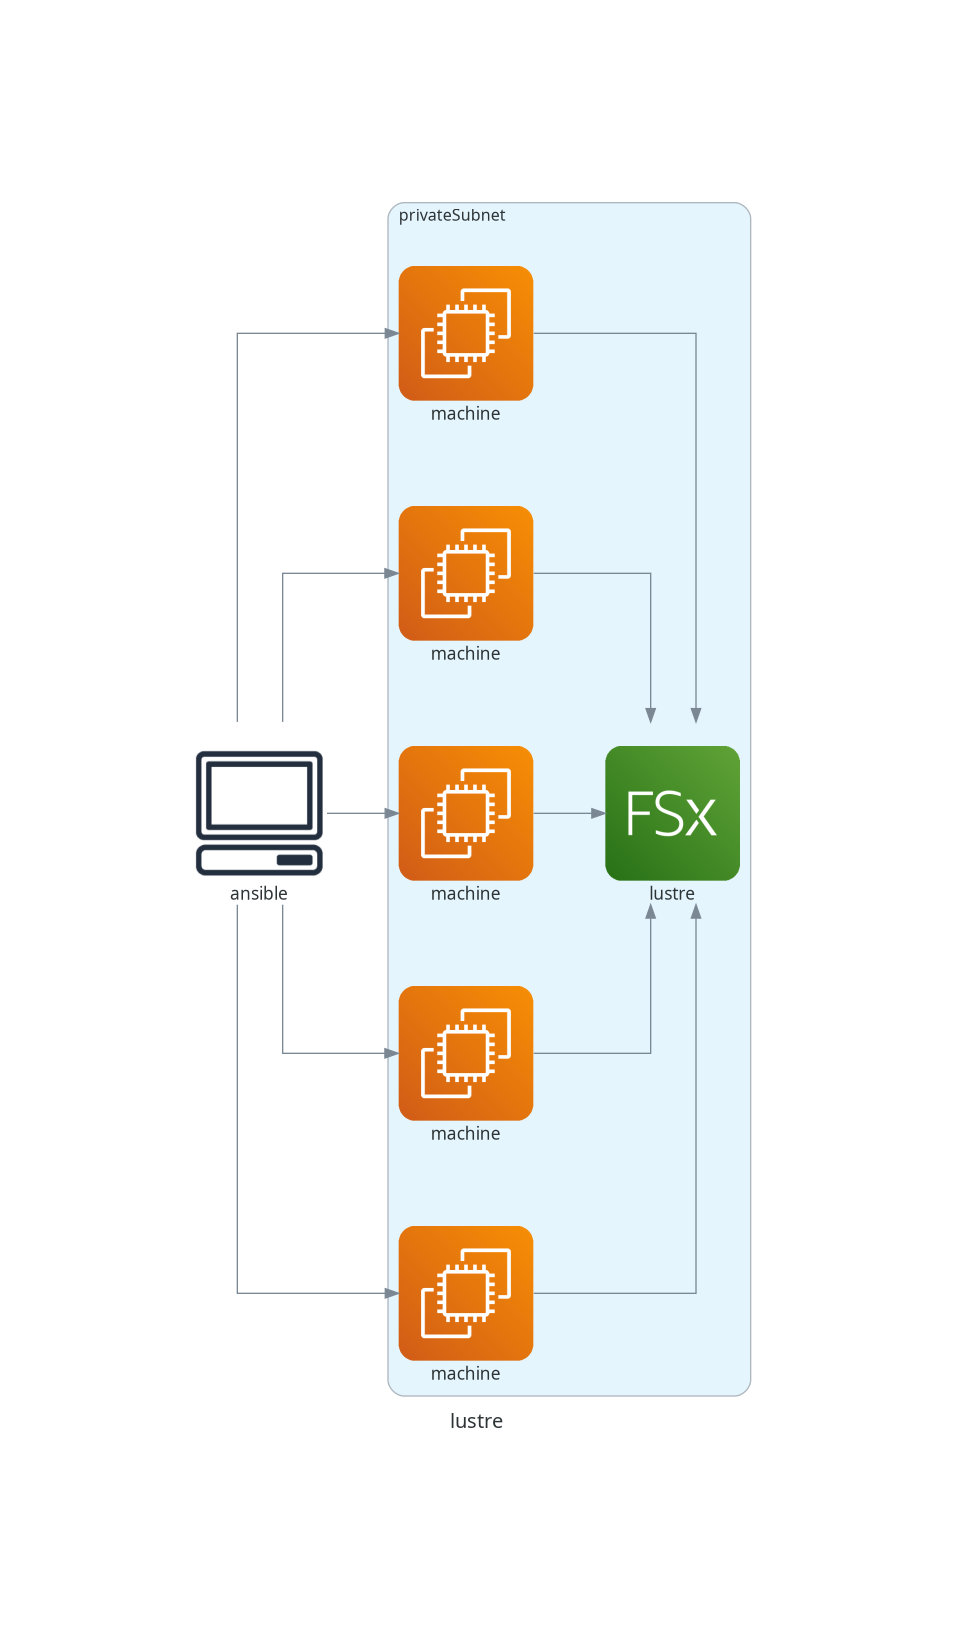
\includegraphics[width=1\textwidth]{lustre.png}
	\caption{Arquitetura do cluster usando lustre Fonte: fornecido pelo autor.}
	\label{fig:lustre}
\end{figure}

\subsection{S3}
Como visto na figura~\ref{fig:s3}., a arquitetura utilizada contém 2 sub-redes, uma privada e uma pública, com as maquinas da subnet privada acessando o bucket s3 provisionado via o serviço s3 da propria AWS. Essa arquitetura foi pensada para manter a mesma estrutura do teste com lustre, de forma que possamos comparar apenas a mudança de armazenamento. O teste foi executado com script runTcc.sh, com seu código em anexo. Os resultados foram

\begin{table}[htb]
	\begin{tabular}{|l|l|l|}
		\hline
		& mdtest & ior \\ \hline
		ior-easy-write    &        &     \\ \hline
		mdtest-easy-write &        &     \\ \hline
		ior-hard-write    &        &     \\ \hline
	\end{tabular}
\end{table}

\begin{figure}[htb]
	\centering
	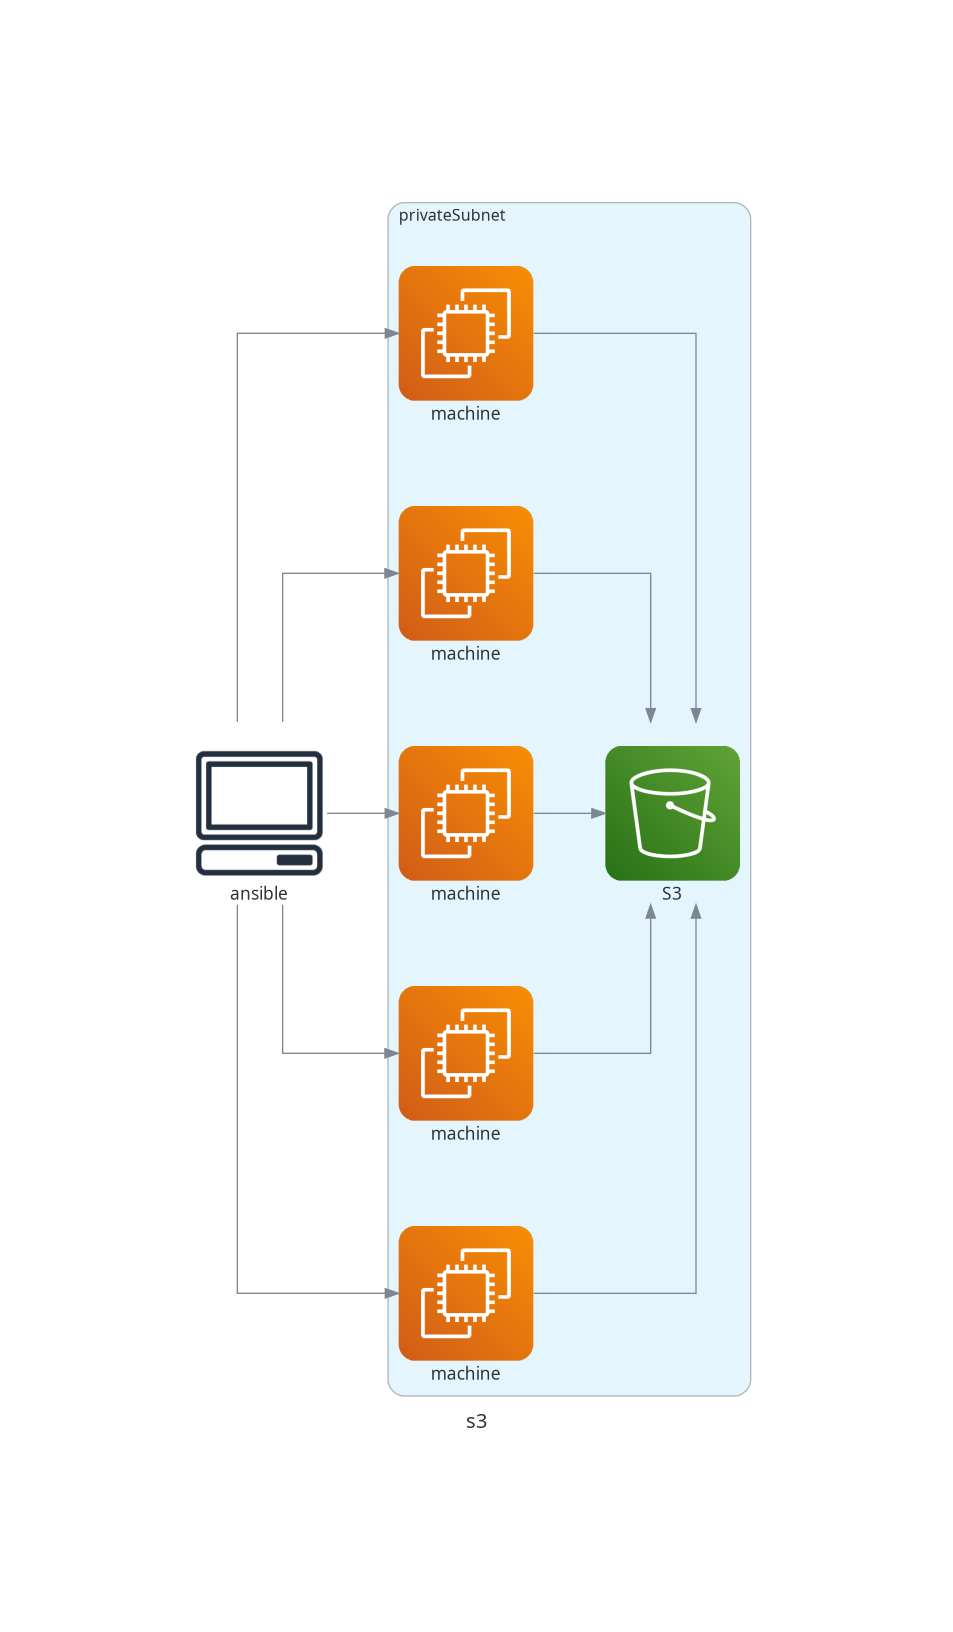
\includegraphics[width=1\textwidth]{s3.png}
	\caption{Arquitetura do cluster usando s3 Fonte: fornecido pelo autor.}
	\label{fig:s3}
\end{figure}

\section{Conclusão}


\newpage
\bibliography{references}

\newpage
\renewcommand{\listfigurename}{APÊNDICE A - Lista de ilustrações}
\listoffigures

\newpage
\renewcommand{\listtablename}{APÊNDICE B - Lista de tabelas}
\listoftables

\begin{appendices}
\newpage
\chapter* {APÊNDICE C}
\noindent
Os apêndices A e B devem conter a lista de ilustrações e tabelas, respectivamente. Os apêndices seguintes podem ser usados para apresentar textos elaborados pelo próprio autor, a fim de complementar a sua argumentação. Por exemplo, no caso de desenvolvimento de sistemas, podem constar nos apêndices os artefatos gerados da análise de sistemas, como protótipos de telas, casos de uso, diagramas UML, ou a lista de requisitos de negócio e de usuário.

\newpage
\chapter*{ANEXO A}
\noindent
Seção opcional. Anexos são os documentos de autoria externa, ou não elaborados pelo autor, que servem de fundamentação, comprovação ou ilustração.
\end{appendices}

\newpage
\chapter*{Agradecimentos}
\noindent
Seção opcional. Oportunidade para o(s) autor(es) registrar(em) os agradecimentos, em especial, quando o artigo recebeu ajuda financeira de alguma instituição de fomento, ou represente o resultado de um trabalho colaborativo ou multidisciplinar, envolvendo áreas externas ao Instituto de Computação.

\end{document}
